

The problem of change point detection appears each time one needs to explore sequence of random data and make a decision about homogeneity of its structure. This could be clarified with two following questions: are there  any structural changes in the nature of observed data? At which moments, if so? Let  $\mathbb{Y} = (Y_1, Y_2,\ldots, Y_n)$ denote the data, ordered by time. Each $Y_i$ has statistical properties defined by some (presumably unknown) $\P_i(Y | Y_{i-1},\ldots,Y_1)$. One says that there is a change points if there exists a time moment $t$ where $\P_t \neq \P_{t+1}$. In online mode with increasing sequence size ($n$) the goal is to detect $t$ as faster as possible minimizing the number of false alarms and missed cases at the same time. In offline mode with fixed sequence size one care about exactitude of change point locations. 

The most frequent application case of change point methods is stochastic model composition from non-fuzzed data split \textbf{[link]}. The alternative case is anomaly registration in a mono-stream observations \textbf{[link]}.    


Our consideration will be restricted by sliding window methods, which calculate some statistic sequentially  and  indicate changes by its critical value surpassing. 
Classical works with such methods are \cite{wm1}, \cite{wm2}.      
There are two the most evident approaches of the critical values calibration. Many existing methods [links] use preliminary information about the nature of data, specification of the type of distribution (true parametric assumption)  or type of change point (change in mean, change in variance e.t.c). These methods obtains critical values as quantiles if the preassumed data distribution. The the way of determining critical values is applying MC resampling procedures, which train on homogeneous region with empirical data distribution.    
This work  contributes into the described window methods in the following items:
\begin{enumerate}
\item MC resampling procedure of the proposed method is shown to be consistent with the reference distribution and the convergence speed is estimated;
\item Training calibration procedure doesn't require  homogeneous regions and could be executed with change pointed data;
\item A novel concept of patterns for different types of changes allows to differ  and correspondingly better indicate abrupt, continuous changes and outliers.    
\end{enumerate}

The geometry of a pattern depends on a type of switch between distributions the data obeys before and after a change respectively. Three examples are presented at the Fig.~\ref{fig:patterns}. The triangle pattern appears in case of an abrupt switch from $\P_{\theta_1^*}$ to $\P_{\theta_2^*}$. A smooth transition between two regimes entails the trapezium change-point pattern. And an inverted triangle pattern appears due to a change in coefficients of linear regression. The control of a change-point pattern instead of a single LRT-value allows to reduce false-alarm rate to zero.

\begin{figure}[!h]
    \centering
    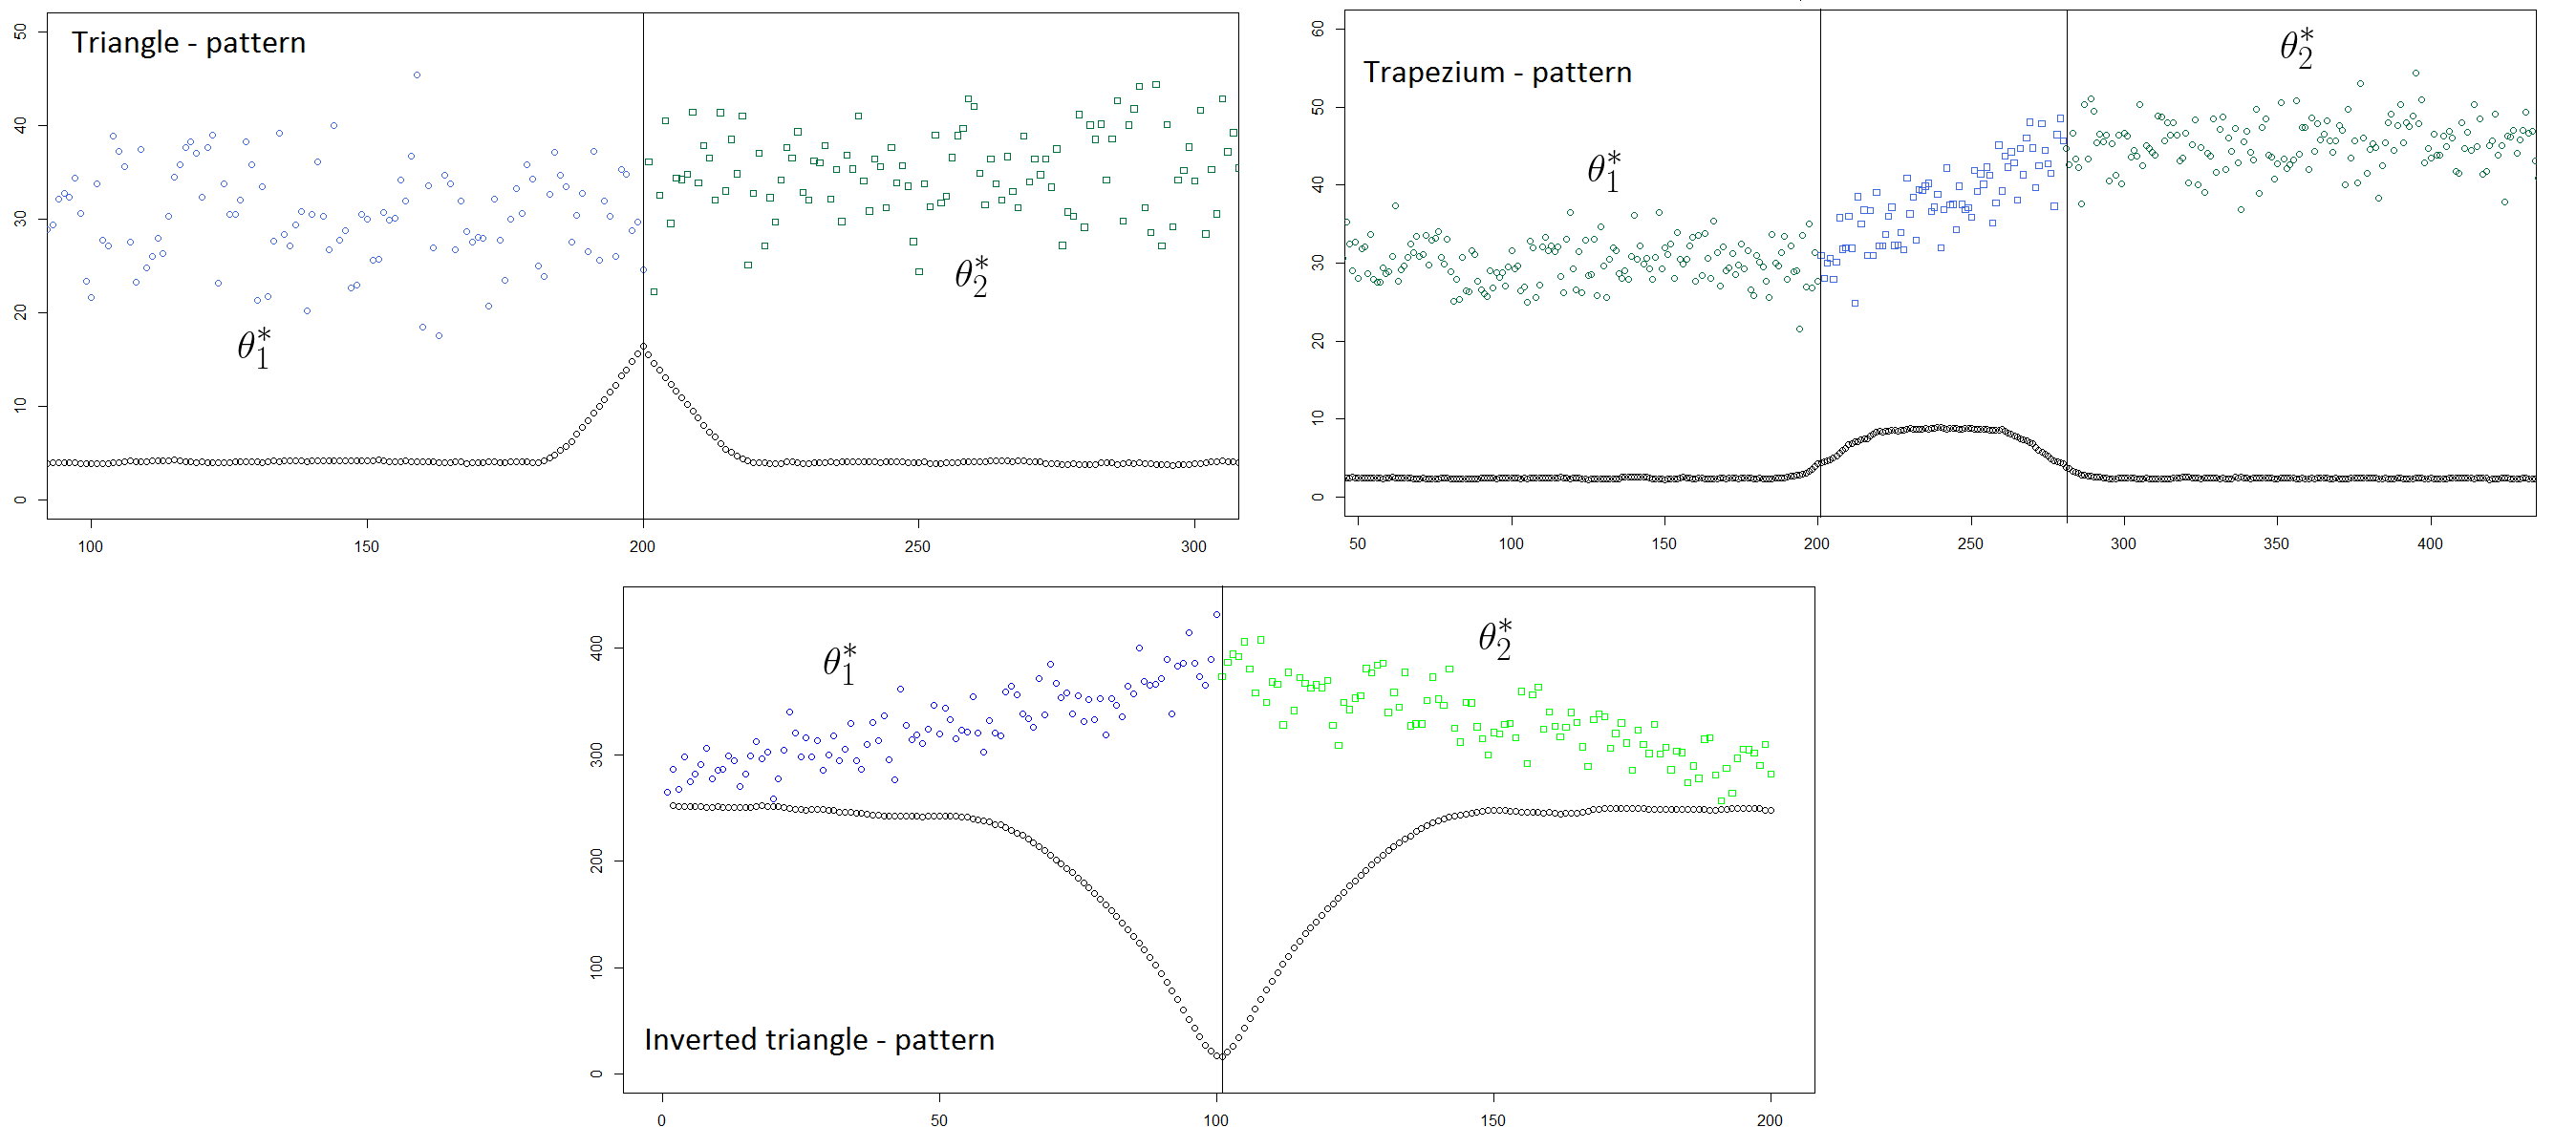
\includegraphics[width=0.5\textwidth, height=0.25\textwidth]{images/patterns-3.png}
    \caption{Type of change point and the geometry of change-point pattern}
    \label{fig:patterns}
\end{figure}


The paper is organized as follows. Section~\ref{sec:procedure} presents the description of the algorithm. Theoretical properties of the procedure and MC resampling are discussed in the next ensuing Sections.  
